\begin{figure*}[t]
    \centering
    \begin{minipage}[t]{0.6\textwidth} % 2/3 width
        \centering
% \vspace{-5mm}
\resizebox{0.33\textwidth}{!}{%
\begin{subfigure}[b]{0.4\textwidth}
    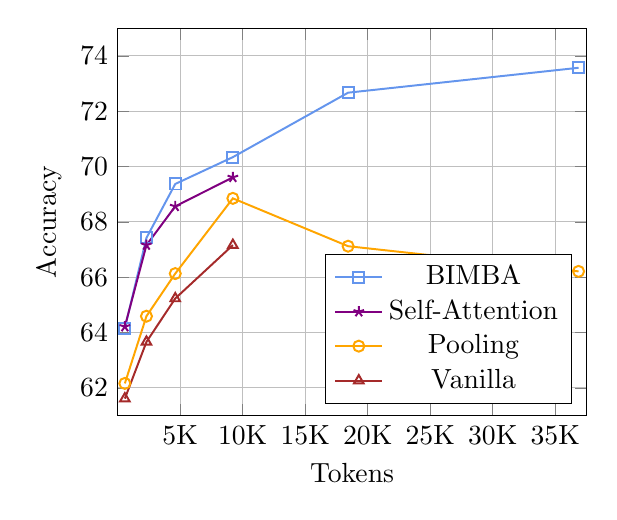
\begin{tikzpicture}
    \begin{axis}[
        % width=12cm, 
        height=6.5cm,
        xlabel={Tokens},
        ylabel={Accuracy},
        %title={(a) LLaVA Backbone on NeXT-QA},
        xmin=0, xmax=37500,
        ymin=61, ymax=75,
        %xtick={576, 2304, 4608, 9216, 18432, 36864},
        % xticklabels={576, 2304, 4608, 9216, 18432, 36864},
        xtick={5000, 10000, 15000, 20000,25000,30000, 35000},
        xticklabels={5K, 10K, 15K, 20K, 25K,30K, 35K},
        ytick={62, 64, 66, 68, 70, 72, 74},
        legend pos=south east,
        grid=both,
        scaled ticks = false,
        scaled x ticks = false,
        % xmode=log,
        % log basis x=1
    ]
    % BIMBA Data
    \addplot[line width=.25mm, color=CornflowerBlue, mark=square, mark size=2pt]
    coordinates {
    (576, 64.16) (2304, 67.42) (4608, 69.37) (9216, 70.34) (18432, 72.67) (36864, 73.57)
    };
    \addlegendentry{BIMBA}
    
    % Self-Attention Data
    \addplot[line width=.25mm, color=Purple, mark=star, mark size=2pt]
        coordinates {
        (576, 64.21) (2304, 67.16) (4608, 68.56) (9216, 69.61)
    };
    \addlegendentry{Self-Attention}
    
    % Pooling Data
    \addplot[line width=.25mm, color=Orange, mark=o, mark size=2pt]
    coordinates {
    (576, 62.16) (2304, 64.59) (4608, 66.13) (9216, 68.85) (18432, 67.12) (36864, 66.21)
    };
    \addlegendentry{Pooling}

    \addplot[line width=.25mm, color=Brown, mark=triangle, mark size=2pt]
    coordinates {
    (576, 61.61) (2304, 63.66) (4608, 65.23) (9216, 67.16) 
    };
    \addlegendentry{Vanilla}
    \end{axis}
    \end{tikzpicture}
    \caption{NExT-QA performance of models based on LLaVA.}
    \vspace{3mm}
\end{subfigure}
}
\hfill
\resizebox{0.33\textwidth}{!}{%
\begin{subfigure}[b]{0.4\textwidth}
    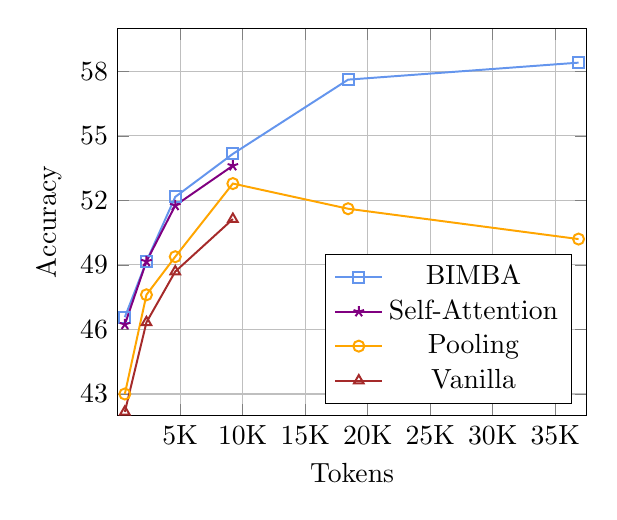
\begin{tikzpicture}
    \begin{axis}[
        % width=12cm, height=8cm,
        %height=7cm,
        height=6.5cm,
        xlabel={Tokens},
        ylabel={Accuracy},
        %title={(b) LLaVA Backbone on EgoSchema},
        xmin=0, xmax=37500,
        ymin=42, ymax=60,
        %xtick={576, 2304, 4608, 9216, 18432, 36864},
        % xticklabels={576, 2304, 4608, 9216, 18432, 36864},
        xtick={5000, 10000, 15000, 20000,25000,30000, 35000},
        xticklabels={5K, 10K, 15K, 20K, 25K,30K, 35K},
        ytick={43, 46, 49, 52, 55, 58, 61},
        legend pos=south east,
        grid=both,
        scaled ticks = false,
        scaled x ticks = false,
        % xmode=log,
        % log basis x=1
    ]
    % BIMBA Data
    \addplot[line width=.25mm, color=CornflowerBlue, mark=square, mark size=2pt]
    coordinates {
    (576, 46.57) (2304, 49.16) (4608, 52.16) (9216, 54.16) (18432, 57.61) (36864, 58.40)
    };
    \addlegendentry{BIMBA}

    % Self-Attention Data
    \addplot[line width=.25mm, color=Purple, mark=star, mark size=2pt]
        coordinates {
        (576, 46.23) (2304, 49.16) (4608, 51.76) (9216, 53.61)
    };
    \addlegendentry{Self-Attention}

    % Pooling Data
    \addplot[line width=.25mm, color=Orange, mark=o, mark size=2pt]
    coordinates {
    (576, 43.00) (2304, 47.61) (4608, 49.38) (9216, 52.78) (18432, 51.61) (36864, 50.20)
    };
    \addlegendentry{Pooling}

    \addplot[line width=.25mm, color=Brown, mark=triangle, mark size=2pt]
    coordinates {
    (576, 42.17) (2304, 46.33) (4608, 48.69) (9216, 51.13) 
    };
    \addlegendentry{Vanilla}
    \end{axis}
    \end{tikzpicture}
    \caption{EgoSchema performance of models based on LLaVA.}
    \vspace{3mm}
\end{subfigure}
}
\resizebox{0.33\textwidth}{!}{%
\begin{subfigure}[b]{0.4\textwidth}
    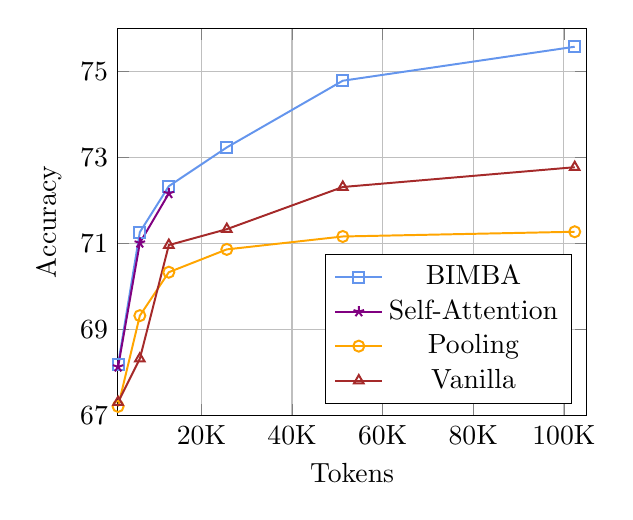
\begin{tikzpicture}
    \begin{axis}[
        % width=12cm, height=8cm,
        %height=7cm,
        height=6.5cm,
        xlabel={Tokens},
        ylabel={Accuracy},
        %title={(a) LLaMA Backbone on NeXT-QA},
        xmin=1500, xmax=105000,
        ymin=67, ymax=76,
        %xtick={1600, 6400, 12800, 25600, 51200, 102400},
        % xticklabels={1600, 6400, 12800, 25600, 51200, 102400},
        xtick={20000,40000,60000,80000,100000},
        xticklabels={20K, 40K, 60K, 80K, 100K},
        ytick={67, 69, 71, 73, 75, 77},
        legend pos=south east,
        grid=both,
        scaled ticks = false,
        scaled x ticks = false,
        % xmode=log,
        % log basis x=1
    ]
    % BIMBA Data
    \addplot[line width=.25mm, color=CornflowerBlue, mark=square, mark size=2pt]
    coordinates {
    (1600, 68.19) (6400, 71.26) (12800, 72.33) (25600, 73.23) (51200, 74.78) (102400, 75.57)
    };
    \addlegendentry{BIMBA}
    
    % Self-Attention Data
    \addplot[line width=.25mm, color=Purple, mark=star, mark size=2pt]
        coordinates {
        (1600, 68.13) (6400, 71.01) (12800, 72.16) 
    };
    \addlegendentry{Self-Attention}
    
    % Pooling Data
    \addplot[line width=.25mm, color=Orange, mark=o, mark size=2pt]
    coordinates {
    (1600, 67.21) (6400, 69.32) (12800, 70.33) (25600, 70.86) (51200, 71.16) (102400, 71.27)
    };
    \addlegendentry{Pooling}
    \addplot[line width=.25mm, color=Brown, mark=triangle, mark size=2pt]
    coordinates {
    (1600, 67.31) (6400, 68.32) (12800, 70.96) (25600, 71.33) (51200, 72.31) (102400, 72.77)
    };
    \addlegendentry{Vanilla}
    \end{axis}
    \end{tikzpicture}
    \caption{NExT-QA performance of models based on LLaMA.}
% \caption{Figure 1}
\end{subfigure}
}
\hfill
\resizebox{0.33\textwidth}{!}{%
\begin{subfigure}[b]{0.4\textwidth}
    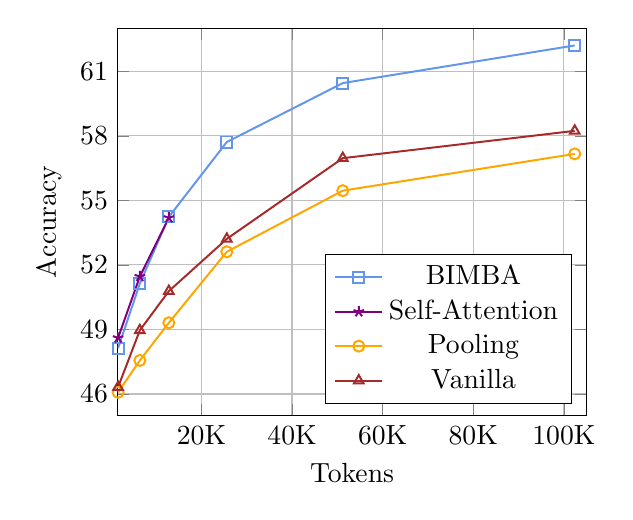
\begin{tikzpicture}
    \begin{axis}[
        % width=12cm, height=8cm,
        height=6.5cm,
        xlabel={Tokens},
        ylabel={Accuracy},
        %title={(b) LLaMA Backbone on EgoSchema},
        xmin=1500, xmax=105000,
        ymin=45, ymax=63,
        %xtick={1600, 6400, 12800, 25600, 51200, 102400},
        % xticklabels={1600, 6400, 12800, 25600, 51200, 102400},
        xtick={20000,40000,60000,80000,100000},
        xticklabels={20K, 40K, 60K, 80K, 100K},
        ytick={46, 49, 52, 55, 58, 61},
        legend pos=south east,
        grid=both,
        scaled ticks = false,
        scaled x ticks = false,
        % xmode=log,
        % log basis x=1
    ]
    % BIMBA Data
    \addplot[line width=.25mm, color=CornflowerBlue, mark=square, mark size=2pt]
    coordinates {
    (1600, 48.13) (6400, 51.13) (12800, 54.23) (25600, 57.71) (51200, 60.45) (102400, 62.20)
    };
    \addlegendentry{BIMBA}
    
    % Self-Attention Data
    \addplot[line width=.25mm, color=Purple, mark=star, mark size=2pt]
        coordinates {
        (1600, 48.61) (6400, 51.46) (12800, 54.19)
    };
    \addlegendentry{Self-Attention}

    % Pooling Data
    \addplot[line width=.25mm, color=Orange, mark=o, mark size=2pt]
    coordinates {
    (1600, 46.08) (6400, 47.56) (12800, 49.31) (25600, 52.61) (51200, 55.45) (102400, 57.16)
    };
    \addlegendentry{Pooling}

    \addplot[line width=.25mm, color=Brown, mark=triangle, mark size=2pt]
    coordinates {
    (1600, 46.32) (6400, 48.96) (12800, 50.78) (25600, 53.21) (51200, 56.96) (102400, 58.23)
    };
    \addlegendentry{Vanilla}
    \end{axis}
    \end{tikzpicture}
    \caption{EgoSchema performance of models based on the LLaMA.}
\end{subfigure}
}
\vspace{-3mm}
\caption{Accuracy achieved by \model { a}nd baseline models on NeXT-QA (left) and EgoSchema (right) as a function of the number of input tokens for models based on LLaVA (top row) and LLaMA (bottom row).  \model { a}chieves the highest accuracy for all sequence lengths and improves monotonically as the number of input tokens is increased. Self-attention cannot be applied to long sequence as it causes an out of memory once the number of tokens becomes too large.}
\vspace{-5mm}
\label{fig:performance}

% \LT{add arrow and ``out of memory''}
% \label{fig:figure1}
\end{minipage}%
    ~ % optional space
\begin{minipage}[t]{0.33\textwidth} % 1/3 width
        \centering
\resizebox{0.4\textwidth}{!}{%
        \begin{subfigure}[b]{0.48\textwidth}
    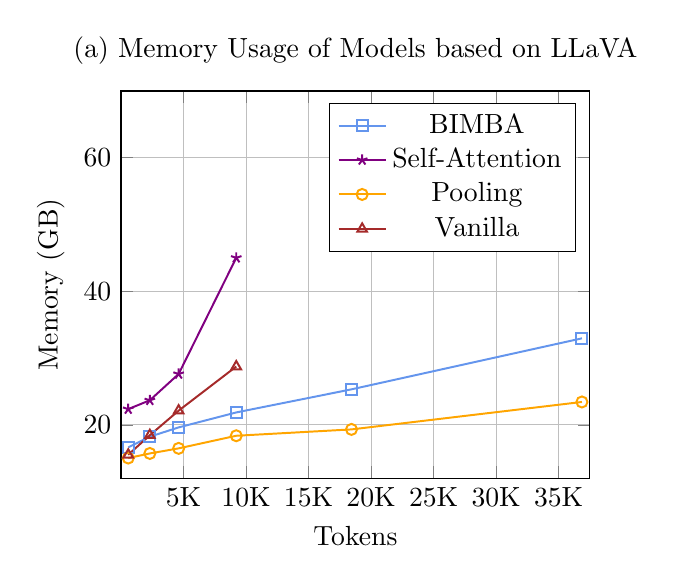
\begin{tikzpicture}
    \begin{axis}[
        % width=12cm, height=8cm,
        height=6.5cm,
        xlabel={Tokens},
        ylabel={Memory (GB)},
        title={(a) Memory Usage of Models based on LLaVA},
        xmin=0, xmax=37500,
        ymin=12, ymax=70,
        %xtick={576, 2304, 4608, 9216, 18432, 36864},
        % xticklabels={576, 2304, 4608, 9216, 18432, 36864},
        xtick={5000, 10000, 15000, 20000,25000,30000, 35000},
        xticklabels={5K, 10K, 15K, 20K, 25K,30K, 35K},
        %ytick={62, 64, 66, 68, 70, 72, 74},
        legend pos=north east,
        grid=both,
        scaled ticks = false,
        scaled x ticks = false,
        % xmode=log,
        % log basis x=1
    ]
    % BIMBA Data
    \addplot[line width=.25mm, color=CornflowerBlue, mark=square, mark size=2pt]
    coordinates {
    (576, 16.62) (2304, 18.22) (4608, 19.61) (9216, 21.85) (18432, 25.31) (36864, 32.95)
    };
    \addlegendentry{BIMBA}
    
    % Self-Attention Data
    \addplot[line width=.25mm, color=Purple, mark=star, mark size=2pt]
        coordinates {
        (576, 22.35) (2304, 23.67) (4608, 27.61) (9216, 45.01)
    };
    \addlegendentry{Self-Attention}
    
    % Pooling Data
    \addplot[line width=.25mm, color=Orange, mark=o, mark size=2pt]
    coordinates {
    (576, 15.02) (2304, 15.71) (4608, 16.47) (9216, 18.36) (18432, 19.31) (36864, 23.42)
    };
    \addlegendentry{Pooling}

    %Vanilla
    \addplot[line width=.25mm, color=Brown, mark=triangle, mark size=2pt]
    coordinates {
    (576, 15.51) (2304, 18.44) (4608, 22.12) (9216, 28.73) 
    };
    \addlegendentry{Vanilla}

    \end{axis}
    \end{tikzpicture}
% \caption{Figure 1}
\end{subfigure}}

\resizebox{0.33\textwidth}{!}{%
\begin{subfigure}[b]{0.4\textwidth}
    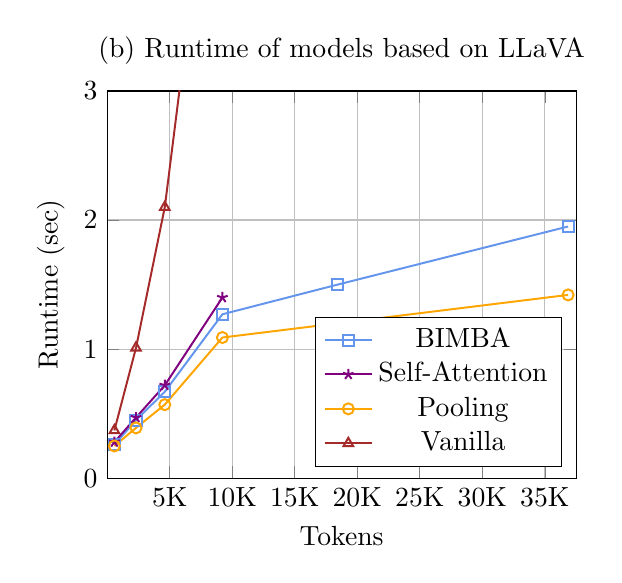
\begin{tikzpicture}
    \begin{axis}[
        % width=12cm, height=8cm,
        height=6.5cm,
        xlabel={Tokens},
        ylabel={Runtime (sec)},
        title={(b) Runtime of models based on LLaVA},
        xmin=0, xmax=37500,
        ymin=0, ymax=3,
        %xtick={576, 2304, 4608, 9216, 18432, 36864},
        % xticklabels={576, 2304, 4608, 9216, 18432, 36864},
        xtick={5000, 10000, 15000, 20000,25000,30000, 35000},
        xticklabels={5K, 10K, 15K, 20K, 25K,30K, 35K},
        %ytick={43, 46, 49, 52, 55, 58, 61},
        legend pos=south east,
        grid=both,
        scaled ticks = false,
        scaled x ticks = false,
        % xmode=log,
        % log basis x=1
    ]
    % BIMBA Data
    \addplot[line width=.25mm, color=CornflowerBlue, mark=square, mark size=2pt]
    coordinates {
    (576, 0.26) (2304, 0.45) (4608, 0.67) (9216, 1.27) (18432, 1.50) (36864, 1.95)
    };
    \addlegendentry{BIMBA}
    
    % Self-Attention Data
    \addplot[line width=.25mm, color=Purple, mark=star, mark size=2pt]
        coordinates {
        (576, 0.28) (2304, 0.47) (4608, 0.72) (9216, 1.40)
    };
    \addlegendentry{Self-Attention}

    % Pooling Data
    \addplot[line width=.25mm, color=Orange, mark=o, mark size=2pt]
    coordinates {
    (576, 0.25) (2304, 0.39) (4608, 0.57) (9216, 1.09) (18432, 1.20) (36864, 1.42)
    };
    \addlegendentry{Pooling}

    %Vanilla
    \addplot[line width=.25mm, color=Brown, mark=triangle, mark size=2pt]
    coordinates {
    (576, 0.37) (2304, 1.01) (4608, 2.10) (9216, 5.65) 
    };
    \addlegendentry{Vanilla}
    
    \end{axis}
    \end{tikzpicture}
    % \caption{Figure 2}
\end{subfigure}
}
\vspace{-3mm}
\caption{Computation cost of \model { a}nd baseline models in terms of memory usage (left) and runtime (right). All models are based on LLaVA. Models based on self-attention or that do not perform compression (Vanilla) run quickly out of memory as the number of input tokens is increased. The runtime of \model { g}rows gracefully as a function of the input sequence length, unlike for the case of Vanilla.}
\vspace{-5mm}
\label{fig:computation llava}
        % \captionof{figure}{Caption for figure 2}
        % \label{fig:figure2}
    \end{minipage}
    % \caption{Overall caption for the figure set}
    % \label{fig:overall}
\end{figure*}